%\documentclass[handout,xcolor=pdftex,dvipsnames,table,mathserif]{beamer}
\documentclass[xcolor=pdftex,dvipsnames,table,mathserif]{beamer}
\usepackage{subfigure}
\usepackage{amsbsy}
\usepackage{tikz}
\usetikzlibrary{arrows}
\usepackage{amsmath,graphicx,dsfont,color}
\usepackage{amsfonts}
\usepackage{amssymb}
\usepackage{array}

\bibliographystyle{apalike}

\setbeamertemplate{bibliography item}{\insertbiblabel}
\setbeamertemplate{bibliography entry title}{}
\setbeamertemplate{bibliography entry location}{}
\setbeamertemplate{bibliography entry note}{}

%Definitiona

\newcommand{\x}{\mathbf{x}}
\newcommand{\X}{\mathbf{X}}
\newcommand{\W}{\mathbf{W}} %Weight
\newcommand{\bais}{\mathbf{b}}%Bais
\newcommand{\act}{\texttt{g}}%Activation
\newcommand{\loss}{L}
\newcommand{\pdata}{\hat{p}_{\texttt{data}}}
\newcommand{\nsize}{n}
\newcommand{\param}{\boldsymbol{\theta}}
\newcommand{\featmap}{\boldsymbol{\phi}}
\newcommand{\EV}{\mathbb{E}}







\usepackage{physics}

\graphicspath{{../graphics/}}

\AtBeginSection[]{
  \begin{frame}{Contents}
    \tableofcontents[currentsection, hideothersubsections]
  \end{frame}
}

\AtBeginSubsection[]{
  \begin{frame}{Contents}
    \tableofcontents[currentsection, subsectionstyle=show/shaded/hide]
  \end{frame}
}

\setbeamertemplate{footline}[frame number]{}
\setbeamertemplate{navigation symbols}{}
\setbeamertemplate{section in toc}[square]
\setbeamertemplate{items}[square]

%% For image credits on image bottom right
\usepackage[absolute,overlay]{textpos}
\setbeamercolor{framesource}{fg=gray}
\setbeamerfont{framesource}{size=\tiny}
\newcommand{\source}[1]{\begin{textblock*}{4cm}(8.7cm,8.6cm)
    \begin{beamercolorbox}[ht=0.5cm,right]{framesource}
      \usebeamerfont{framesource}\usebeamercolor[fg]{framesource} Credits: {#1}
    \end{beamercolorbox}
\end{textblock*}}



\title{Attention and transformers}
\author{E. Decencière}
\date{Mines Paris\\
  PSL Research University\\
  Center for Mathematical Morphology
}
\titlegraphic{
\includegraphics[height=1.7cm]{../graphics/logoemp}}

\useinnertheme{rounded}
\usecolortheme{rose}

%%%%%%%%%%%%%%%%%%%%%%%%%%%%%%%%%%%%%%%%%%%%%%%%%%%%%%%
%%%%%%%%%%%%%%%%%%%%%%%%%%%%%%%%%%%%%%%%%%%%%%%%%%%%%%%

\begin{document}

\frame{\titlepage}

\frame{
  \frametitle{Contents}
  \tableofcontents[hidesubsections]
}

%%%%%%%%%%%%%%%%%%%%%%%%%%%%%%%%%%%%%%%%%%%%%%%%%%
%%%%%%%%%%%%%%%%%%%%%%%%%%%%%%%%%%%%%%%%%%%%%%%%%%
\section{Introduction}


%%%%%%%%%%%%%%%%%%%%%%%%%%%%%%%%%%%%
\begin{frame}{Transformers: a new revolution in deep learning?}

\begin{itemize}
\item Transformers~\cite{vaswani_attention_2017} have brought a break-through in natural language processing
  \item They contribute to the development of new natural language processing applications (translation, voice assistants, etc.)
  \item Will they do the same in image analysis?
\end{itemize}

\vspace{1em}

\scriptsize{NB: Our aim through this lesson is to review the main ideas on attention and transformers, through selected examples. However, this overview is not exhaustive.}

\end{frame}


%%%%%%%%%%%%%%%%%%%%%%%%%%%%%%%%%%%%
\begin{frame}{What are transformers?}

\begin{block}{Definition}
A transformer is a neural network architecture module that allows the network to \alert{adaptively focus its attention} on certain regions of the data.
\end{block}

\pause

\begin{alertblock}{Transformers today}
  Nowadays, when people refer to the transformer, they generally mean the architecture proposed by Vaswani \textit{et al.} in 2017~\cite{vaswani_attention_2017}.
\end{alertblock}

\end{frame}


%%%%%%%%%%%%%%%%%%%%%%%%%%%%%%%%%%%%
%%%%%%%%%%%%%%%%%%%%%%%%%%%%%%%%%%%%
\section{Visual attention}

%%%%%%%%%%%%%%%%%%%%%%%%%%%%%%%%%%%%
\subsection{Attention in human vision}


%%%%%%%%%%%%%%%%%%%%%%%%%%%%%%%%%%%%
\begin{frame}{How do we look at an  image?}

\begin{figure}[ht]
  \centering
  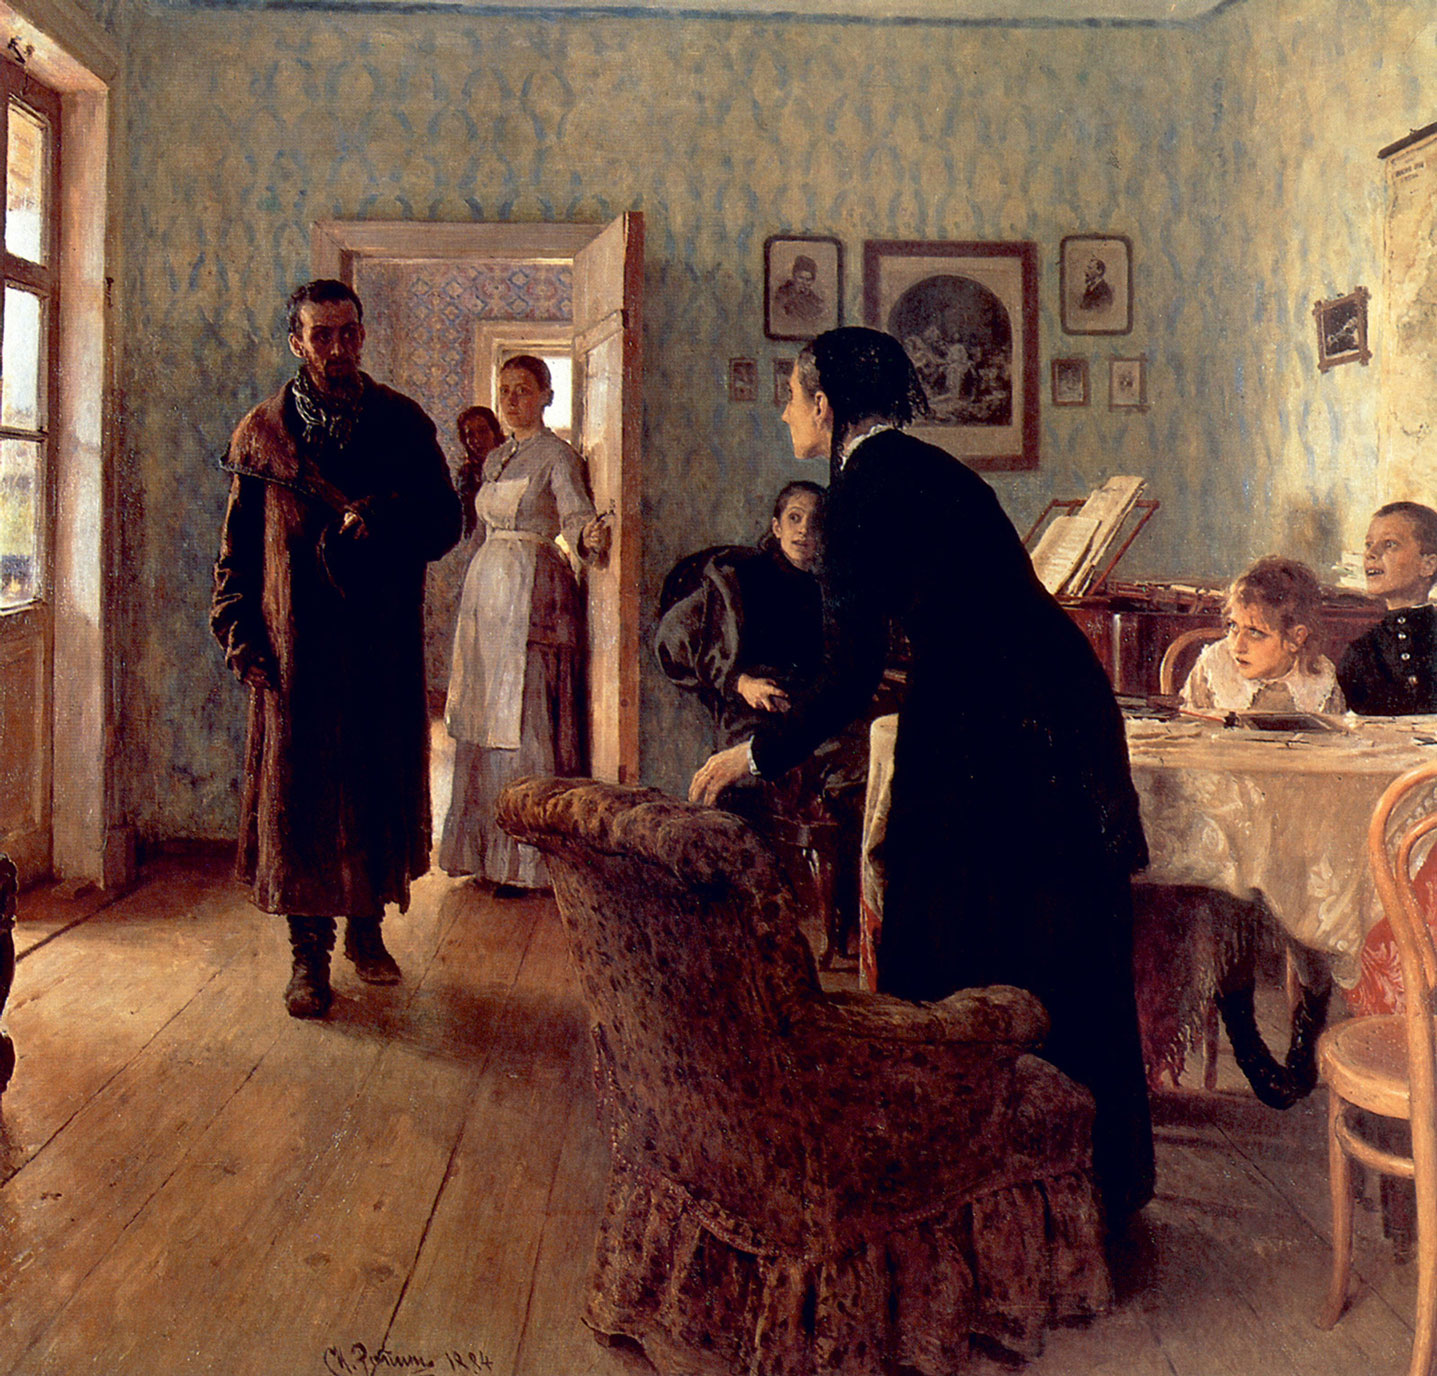
\includegraphics[width=0.6\textwidth]{repin_unexpected_visitor}
  \source{Ilya Repin, An Unexpected Visitor, 1884.}
\end{figure}

\end{frame}


%%%%%%%%%%%%%%%%%%%%%%%%%%%%%%%%%%%%
\begin{frame}{How do we look at an image?}

\begin{figure}[ht]
  \centering
  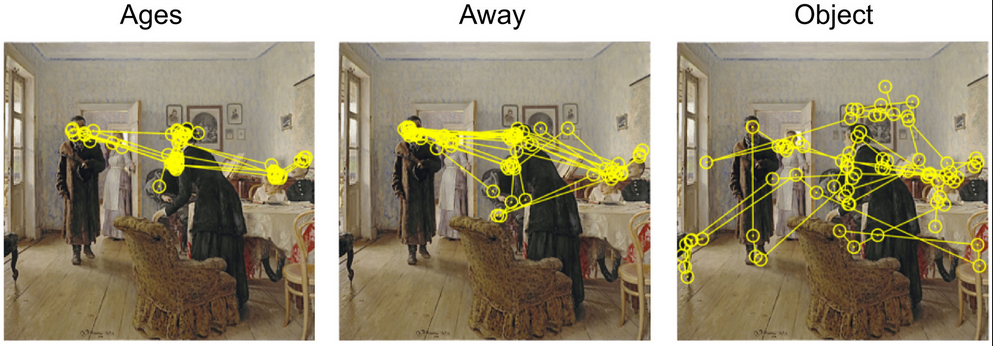
\includegraphics[width=\textwidth]{Yarbus}
    \source{Experiments on visual attention \cite{yarbus_eye_1967}}
\end{figure}

Tasks:
\begin{itemize}
\item Age of the characters?
\item How long has the visitor been away?
\item Memorize the objects in the scene.
\end{itemize}

\end{frame}

%%%%%%%%%%%%%%%%%%%%%%%%%%%%%%%%%%%%
\begin{frame}{Information used by human visual attention}

  \begin{itemize}
  \item Bottom-up:
    \begin{itemize}
    \item local features (orientation, intensity, junctions, colour, motion, etc.)
    \item local features contrast
    \item context
    \end{itemize}
\item Top-bottom: task related
\item Construction of a single \textit{saliency map}

  \end{itemize}

\end{frame}


%%%%%%%%%%%%%%%%%%%%%%%%%%%%%%%%%%%%
\begin{frame}{Exploring the image}


\begin{columns}
  \begin{column}{.5\textwidth}
    \begin{figure}[ht]
      \centering
      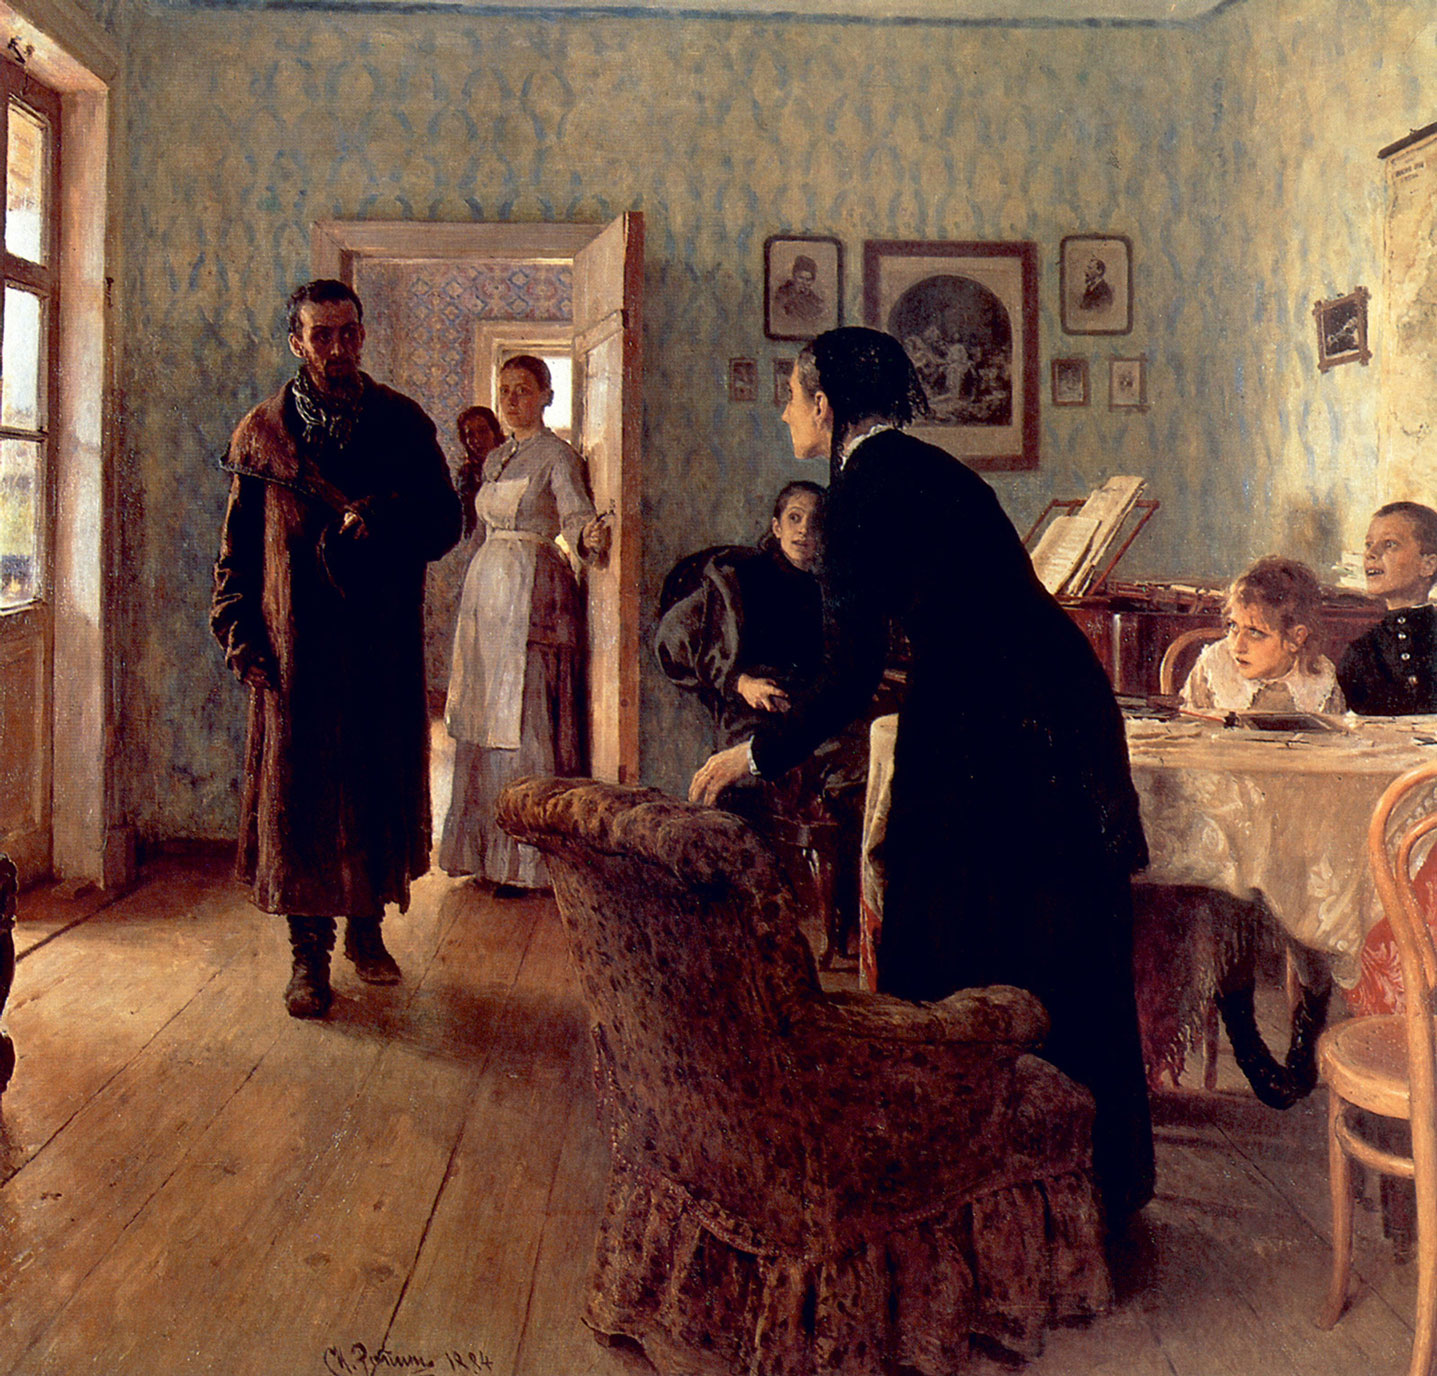
\includegraphics[width=0.9\textwidth]{repin_unexpected_visitor}
    \end{figure}
  \end{column}

  \begin{column}{.5\textwidth}

    \begin{itemize}
  \item Winner-takes all! We focus on the maximum of the saliency map.
  \item Inhibition of return: We explore the following maxima, at first avoiding those that have already been inspected
  \end{itemize}

  \end{column}
\end{columns}


\end{frame}


%%%%%%%%%%%%%%%%%%%%%%%%%%%%%%%%%%%%
\begin{frame}{Why has visual attention evolved?}

  \begin{itemize}
  \item Photoreceptor cells are expensive
  \item Processing power is limited
  \item Solution: concentrate the cells in a given region and use the gaze to optimize their use
  \end{itemize}

\pause

  \begin{alertblock}{}
    \begin{itemize}
    \item The same arguments apply to artificial visual systems
    \item[\textbf{+}] Some degree of invariance
    \item[\textbf{+}] Interpretability
    \end{itemize}
  \end{alertblock}

\end{frame}


%%%%%%%%%%%%%%%%%%%%%%%%%%%%%%%%%%%%
\subsection{Attention in image analysis}

%%%%%%%%%%%%%%%%%%%%%%%%%%%%%%%%%%%%
\begin{frame}{A classical bottom-up model}

\begin{columns}
  \begin{column}{.4\textwidth}
\begin{itemize}
\item Itti et al.~\cite{itti_model_1998} proposed a model inspired by the primate visual system.
\item It only uses low-level information.
\end{itemize}


  \end{column}

  \begin{column}{.6\textwidth}
\begin{figure}[ht]
  \centering
  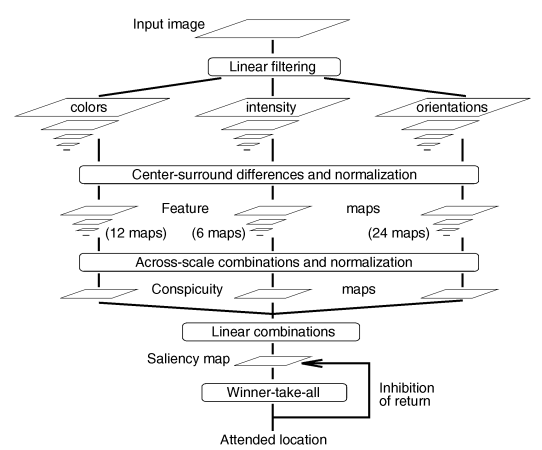
\includegraphics[width=\textwidth]{visual_attention_model_itti}
\end{figure}

  \end{column}
\end{columns}



\end{frame}

%%%%%%%%%%%%%%%%%%%%%%%%%%%%%%%%%%%%
%% \begin{frame}{A bottom-up model}

%% \begin{figure}[ht]
%%   \centering
%%   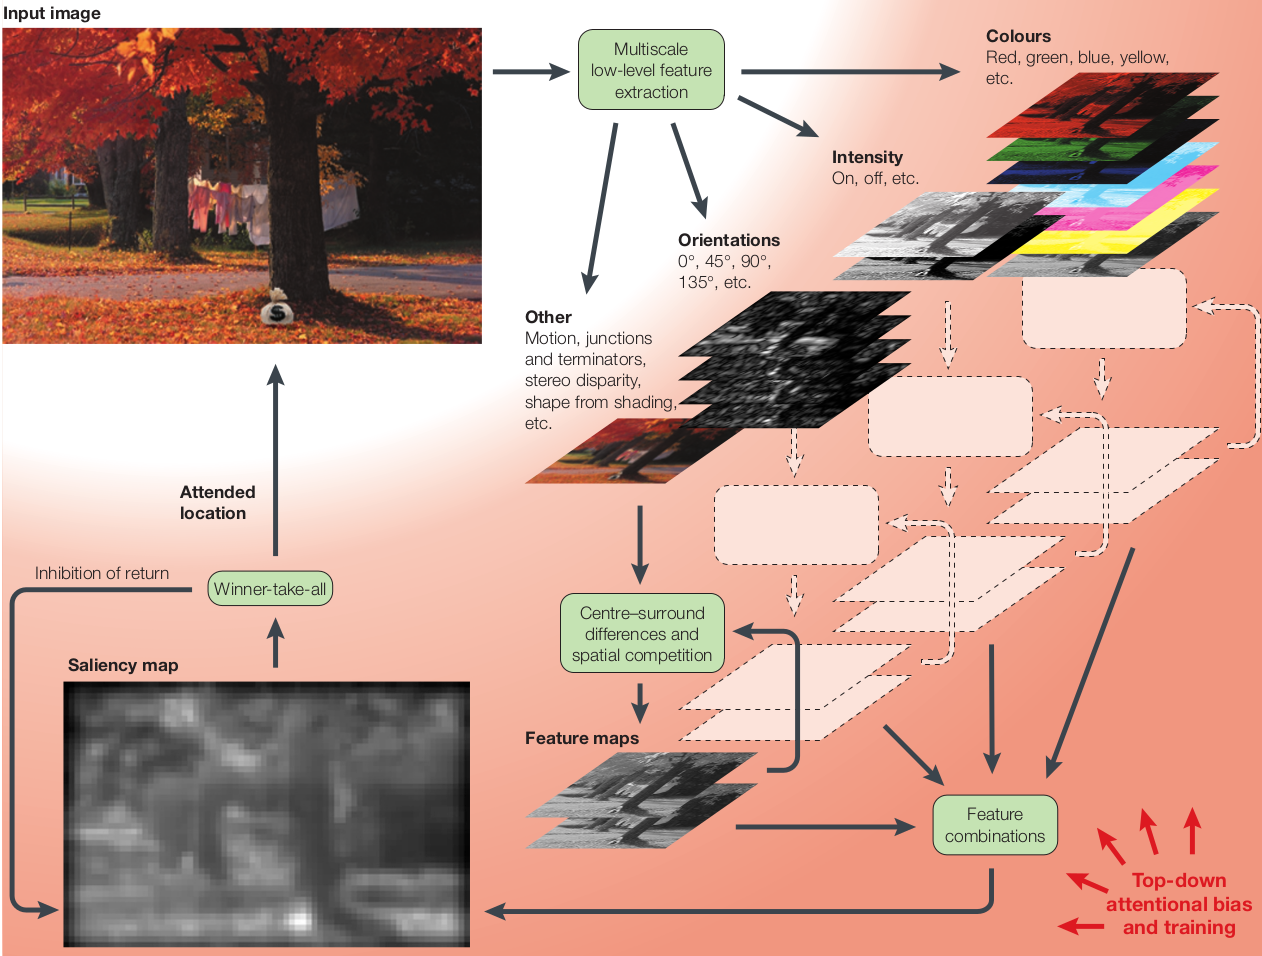
\includegraphics[width=0.9\textwidth]{koch_ullman}
%%   \source{\cite{itti_computational_2001}}
%% \end{figure}


%% \end{frame}


%%%%%%%%%%%%%%%%%%%%%%%%%%%%%%%%%%%%
\begin{frame}{Examples \cite{itti_model_1998}}

\begin{figure}[ht]
  \centering
  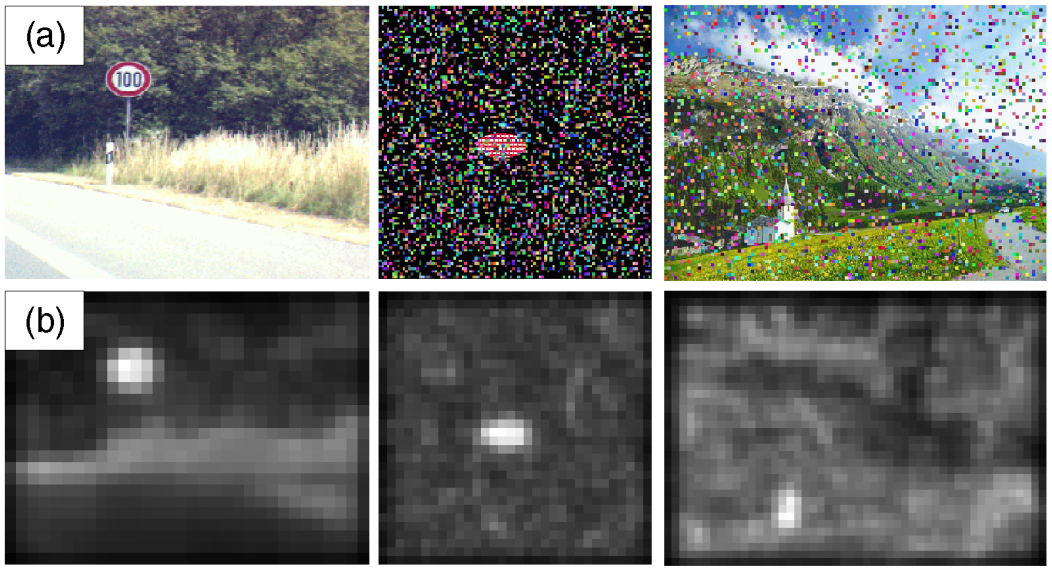
\includegraphics[width=\textwidth]{saliency_maps_itti}
\end{figure}


\end{frame}

%%%%%%%%%%%%%%%%%%%%%%%%%%%%%%%%%%%%
%% \begin{frame}{Top-down attention models}

%%   \begin{itemize}
%%   \item These are task-dependant.
%%   \item Note that all detection methods can be considered as task-oriented attention methods
%%   \end{itemize}

%%   \begin{block}{Example: Face detection with the Viola-Jones method~\cite{viola_rapid_2001}}
%%     \begin{itemize}
%%     \item Define weak learners based on integrals on rectangles
%%     \item Select learners using AdaBoost
%%     \item Apply them in a hierarchical way
%%     \end{itemize}

%% \begin{figure}[ht]
%%   \centering
%%   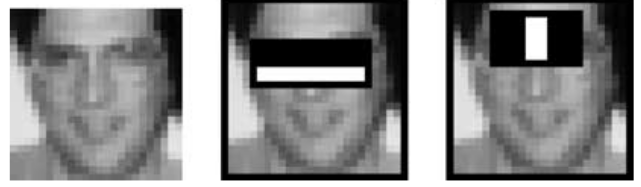
\includegraphics[width=0.7\textwidth]{viola_jones_features}\\
%%   \scriptsize{Image size: $24 \times 24$ pixels}
%% \end{figure}


%%   \end{block}

%% \end{frame}

%% %%%%%%%%%%%%%%%%%%%%%%%%%%%%%%%%%%%%
%% \begin{frame}{Illustration~\cite{viola_rapid_2001}}

%% \begin{figure}[ht]
%%   \centering
%%   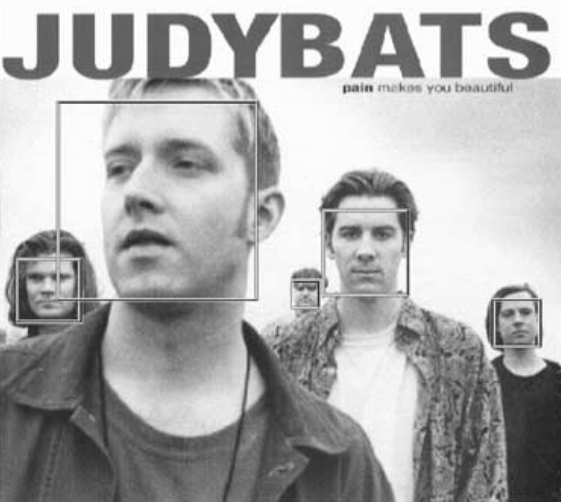
\includegraphics[width=0.6\textwidth]{viola_jones_example}
%% \end{figure}

%% Once attention is focused, the corresponding regions can be further analysed. Here, for identification purposes, for example.

%% \end{frame}


%%%%%%%%%%%%%%%%%%%%%%%%%%%%%%%%%%%%
\subsection{Attention with deep learning}



%%%%%%%%%%%%%%%%%%%%%%%%%%%%%%%%%%%%
\begin{frame}{Region proposal networks \cite{ren_faster_2015}}

  \begin{itemize}
  \item Detection and instance segmentation methods use region proposal networks, that can be interpreted as an attention mechanism.
  \item The region proposal network gives the coordinates of the rectangle and a probability that it contains an object.
  \end{itemize}


\begin{figure}
  \centering
  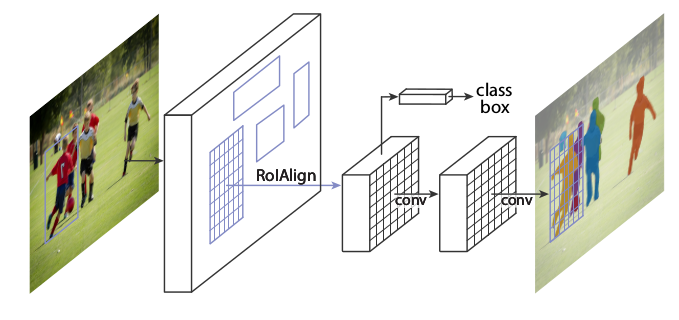
\includegraphics[width=7.5cm]{mask_r_cnn.png}\\
  \scriptsize{A region proposal module is used by mask R-CNN~\cite{he_mask_2017}}
  \end{figure}

\end{frame}


%%%%%%%%%%%%%%%%%%%%%%%%%%%%%%%%%%%%
\begin{frame}{Spatial transformers~\cite{jaderberg_spatial_2016}}

  \begin{columns}
    \begin{column}{.75\textwidth}
      \begin{figure}[ht]
        \centering
        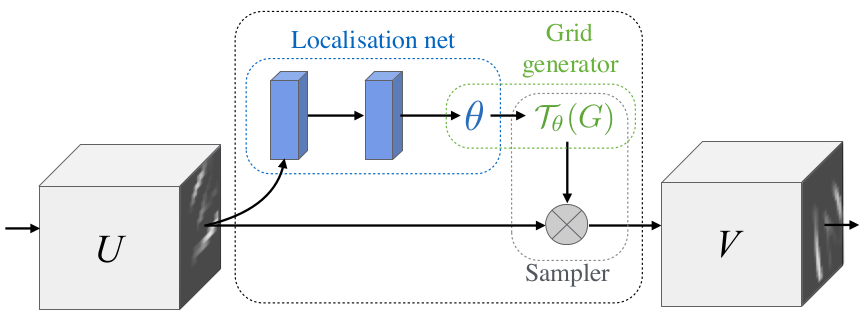
\includegraphics[width=\textwidth]{spatial_transformer}
      \end{figure}

    \end{column}

\pause

    \begin{column}{.25\textwidth}
      \begin{figure}[ht]
        \centering
        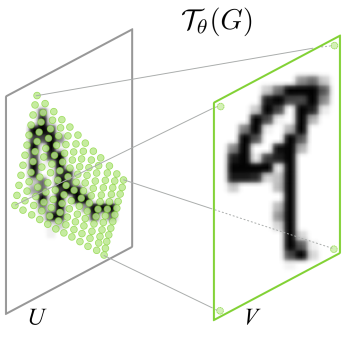
\includegraphics[width=\textwidth]{sampling_grid}
      \end{figure}
    \end{column}
  \end{columns}

\pause

  \vspace{1cm}

  \begin{block}{}
    \begin{itemize}
    \item This module can be added to any convolutional network
    \item End-to-end learning
    \end{itemize}


  \end{block}



\end{frame}

%%%%%%%%%%%%%%%%%%%%%%%%%%%%%%%%%%%%
\begin{frame}{Spatial transformers illustration}

  \begin{figure}[ht]
    \centering
    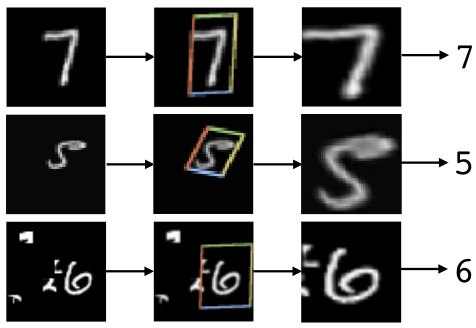
\includegraphics[width=0.7\textwidth]{spatial_transformer_res}
  \end{figure}
\end{frame}

%%%%%%%%%%%%%%%%%%%%%%%%%%%%%%%%%%%%
\begin{frame}{Spatial transformers with multiple heads}

  \begin{figure}[ht]
    \centering
    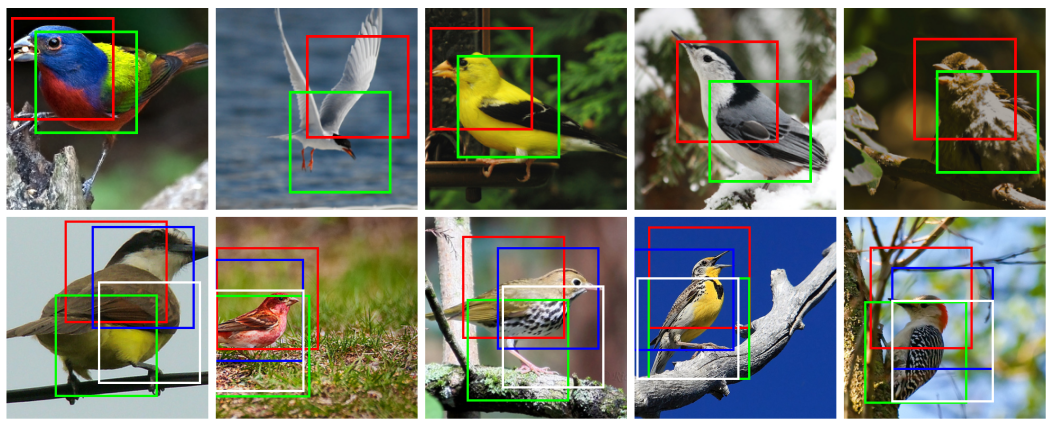
\includegraphics[width=\textwidth]{spatial_transformers_birds}
  \end{figure}

\begin{block}{Remarks}
  \begin{itemize}
  \item Note that in the first row one transformer tends to focus on the bird's head, while the second is centered on the body
  \item In the second row, the specialization is less apparent
  \end{itemize}
\end{block}

\end{frame}

%%%%%%%%%%%%%%%%%%%%%%%%%%%%%%%%%%%%
%%%%%%%%%%%%%%%%%%%%%%%%%%%%%%%%%%%%
\section{The transformer architecture and its applications in computer vision}


%%%%%%%%%%%%%%%%%%%%%%%%%%%%%%%%%%%%
\begin{frame}{Transformer avatars}

  \begin{block}{Some examples}
    \begin{itemize}
    \item Graph transformers~\cite{lecun_gradient-based_1998}
    \item Transforming auto-encoders~\cite{hinton_transforming_2011}
    \item Spatial transformers~\cite{jaderberg_spatial_2016}
    \end{itemize}
  \end{block}

  \begin{alertblock}{\textbf{The} transformer~\cite{vaswani_attention_2017}.}
    Today, when people refer to the transformer, they generally mean the architecture proposed by Vaswani et al. in 2017.
  \end{alertblock}

\end{frame}

%%%%%%%%%%%%%%%%%%%%%%%%%%%%%%%%%%%%
\subsection{The transformer for natural language processing}




%%%%%%%%%%%%%%%%%%%%%%%%%%%%%%%%%%%%
\begin{frame}{The rise of transformers}

  \begin{columns}

    \begin{column}{.5\textwidth}
      \begin{block}{The paper that started it all}
        Vaswani et al., Attention is all you need, Neurips 2017.
      \end{block}
      This architecture was developed for text processing.\\
\vspace{2em}
        NB: the first general differentiable attention mechanism was published in 2015~\cite{bahdanau_neural_2015}.

    \end{column}

    \begin{column}{.5\textwidth}
      \begin{figure}[ht]
        \centering
        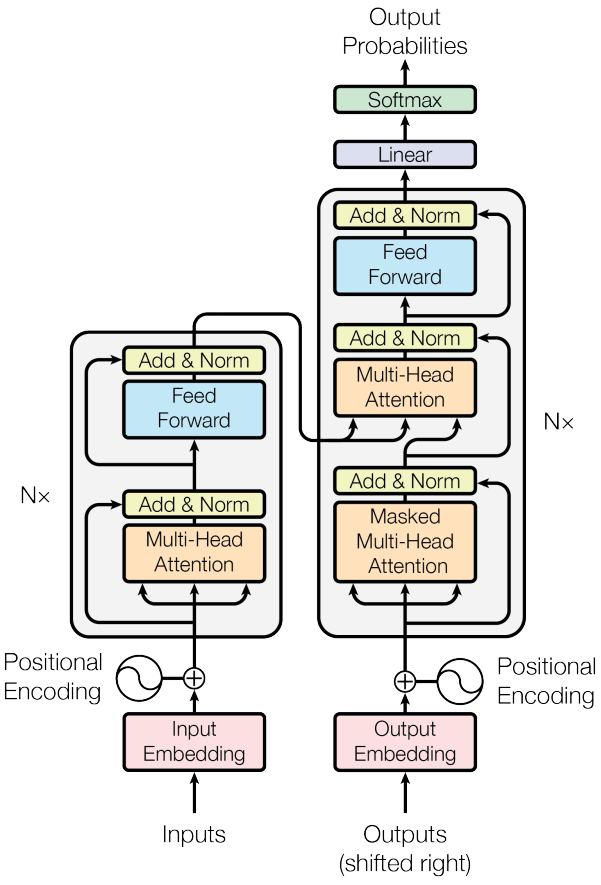
\includegraphics[width=\textwidth]{transformer}
      \end{figure}
    \end{column}

  \end{columns}


\end{frame}

%%%%%%%%%%%%%%%%%%%%%%%%%%%%%%%%%%%%
\begin{frame}{Architecture~\cite{vaswani_attention_2017}}

\begin{figure}[ht]
  \centering
  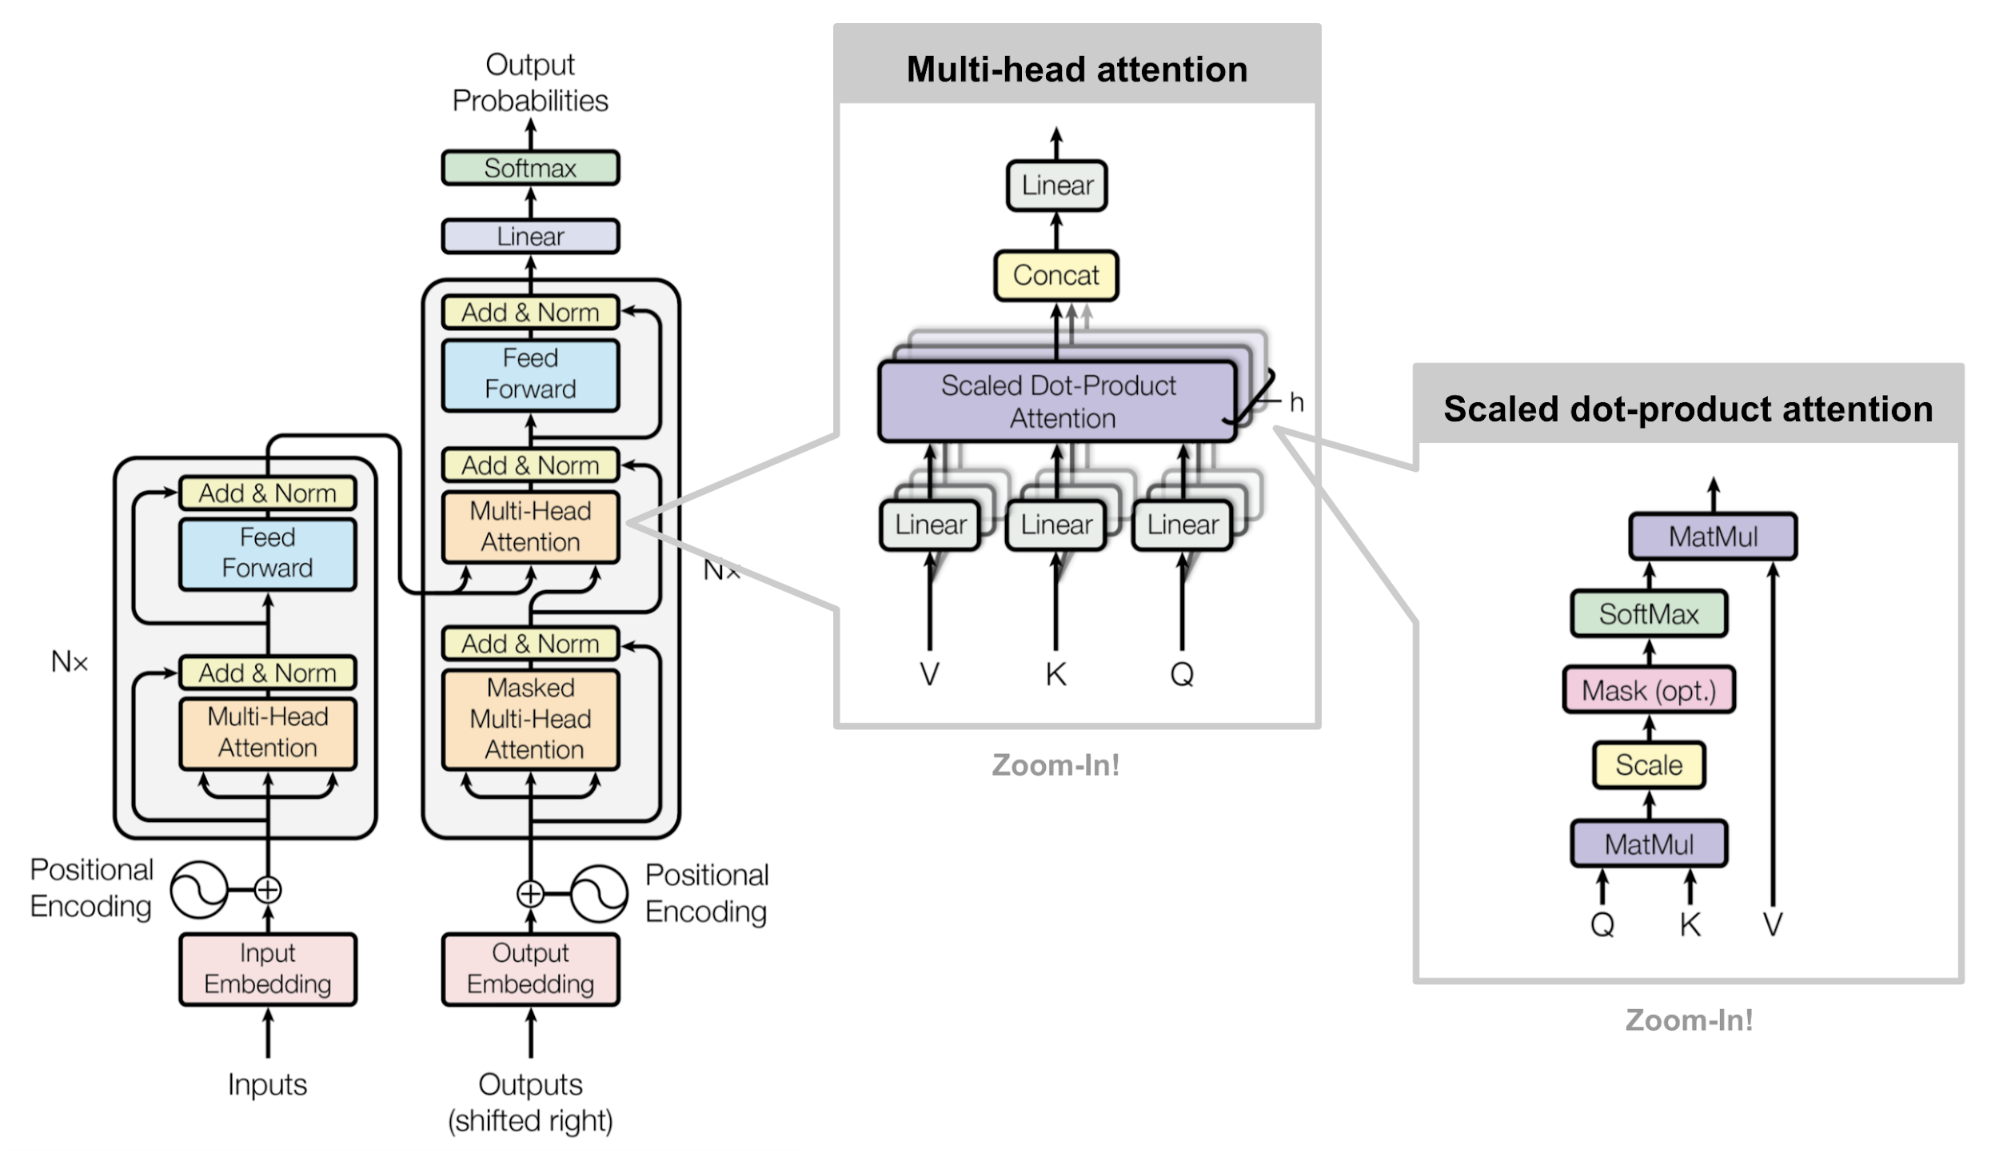
\includegraphics[width=\textwidth]{transformer_with_zooms}
  \source{\url{https://lilianweng.github.io/lil-log/2018/06/24/attention-attention.html}}
\end{figure}


\end{frame}

%%%%%%%%%%%%%%%%%%%%%%%%%%%%%%%%%%%%
\begin{frame}{Scaled dot-product attention}

  \begin{block}{Definition}
    \[Att(Q,K,V) = \sigma\left(\frac{QK^t}{\sqrt{d_{K}}}\right) V \]
  \end{block}

  \begin{itemize}
  \item $V$: values; $K$: keys; $Q$: queries.
  \item $d_{K}$ is the length of $K$.
  \item $\sigma$: row-wise soft-max.
  \end{itemize}


\end{frame}



%%%%%%%%%%%%%%%%%%%%%%%%%%%%%%%%%%%%
\begin{frame}{Self-attention}

  \begin{figure}[ht]
    \centering
    
\includegraphics[width=0.6\textwidth]{self_attention}
  \end{figure}


\end{frame}


%%%%%%%%%%%%%%%%%%%%%%%%%%%%%%%%%%%%
\begin{frame}{Multi-head attention}


\begin{columns}
  \begin{column}{.5\textwidth}
  \begin{figure}[ht]
    \centering
    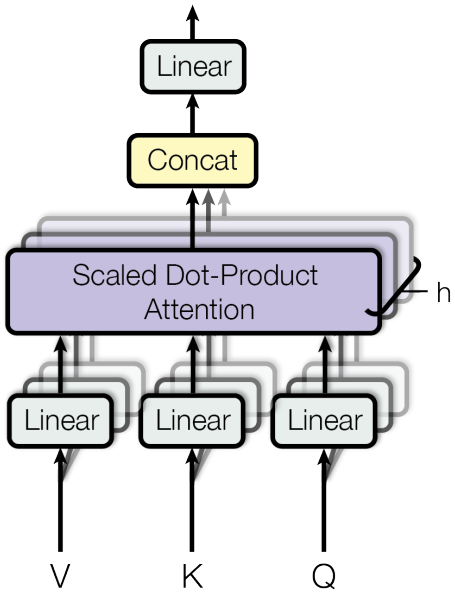
\includegraphics[width=0.55\textwidth]{multi_head_attention}
  \end{figure}

  \end{column}

  \begin{column}{.5\textwidth}
  \begin{itemize}
  \item Matrices $W_Q$, $W_V$ and $W_V$ are learnable.
  \item $h$ heads work in parallel.
  \end{itemize}

  \end{column}
\end{columns}

  %% \begin{block}{Application of scaled dot-product attention}
  %%   %% \[Att(W_QQ,W_KK,W_VV) = \sigma\left(\frac{W_QQ(W_KK)^t}{\sqrt{d_{K'}}}\right) VW_V \]
  %%   %% \[ = \sigma\left(\frac{Q'(K')^t}{\sqrt{d_{K'}}}\right) V' \]
  %%   \begin{align*}
  %%   Att(W_QQ,W_KK,W_VV) & = & \sigma\left(\frac{W_QQ(W_KK)^t}{\sqrt{d_{K'}}}\right) VW_V \\
  %%    & = & \sigma\left(\frac{Q'(K')^t}{\sqrt{d_{K'}}}\right) V'
  %%   \end{align*}
  %% \end{block}


\end{frame}


%%%%%%%%%%%%%%%%%%%%%%%%%%%%%%%%%%%%
%% \begin{frame}{Dot-product self-attention illustration}

%% \begin{columns}
%%   \begin{column}{.4\textwidth}
%%   \begin{figure}[ht]
%%     \centering
%%     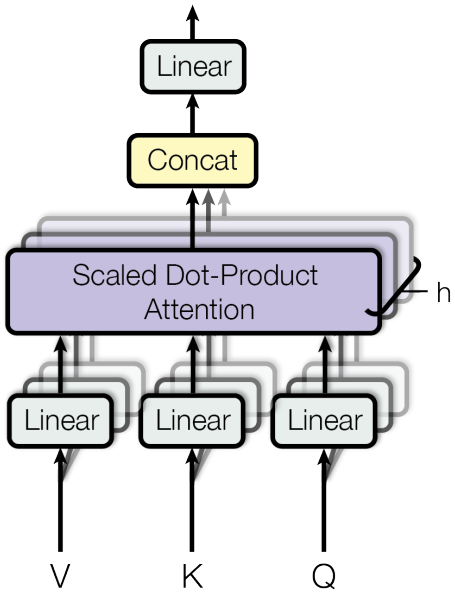
\includegraphics[width=0.6\textwidth]{multi_head_attention}
%%   \end{figure}

%%   \end{column}

%%   \begin{column}{.6\textwidth}
%%     In the case of self-attention:
%%   \begin{itemize}
%%   \item $V = K = Q = X$
%%   \end{itemize}

%%   \end{column}
%% \end{columns}

%% \begin{figure}[ht]
%%   \centering
%%   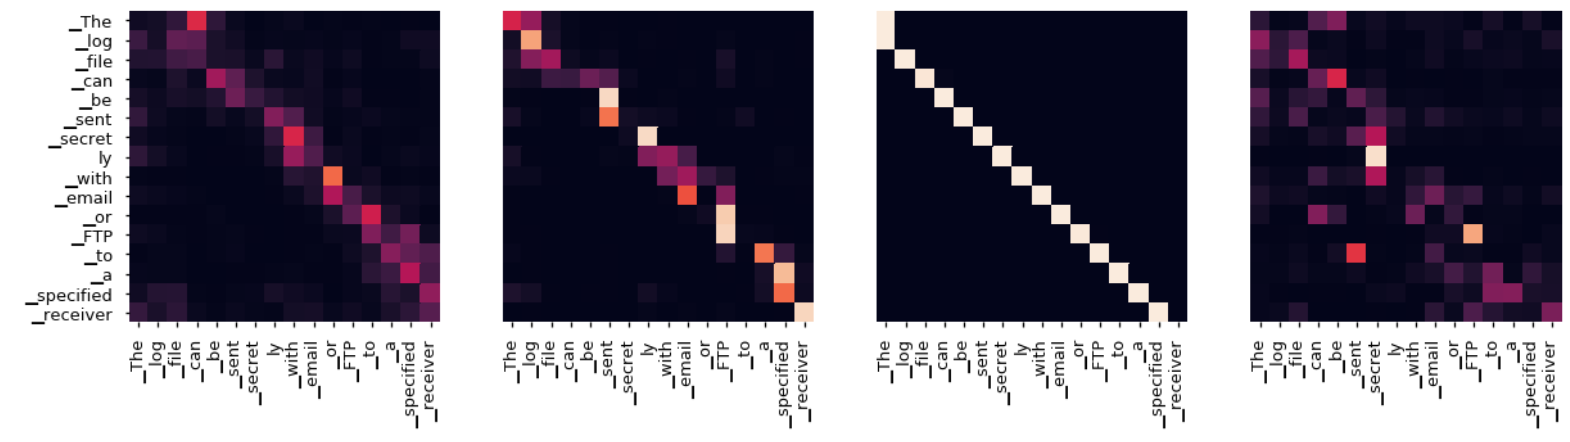
\includegraphics[width=\textwidth]{dot_prod_attention_illustration}
%%   \source{https://nlp.seas.harvard.edu/2018/04/03/attention.html}
%% \end{figure}


%% \end{frame}

%%%%%%%%%%%%%%%%%%%%%%%%%%%%%%%%%%%%
\begin{frame}{Success of transformers in natural language processing}

  \begin{itemize}
  \item Bidirectional Encoder Representations from Transformers (BERT, by Google~\cite{brown_language_2020})
  \item Generative Pre-trained Transformer 3 (GPT-3, by OpenAI~\cite{devlin_bert_2019}): 175 billion parameters.
  \item Generative Pre-trained Transformer 4 (2023) : undisclosed number of parameters.

  \end{itemize}
\end{frame}


%%%%%%%%%%%%%%%%%%%%%%%%%%%%%%%%%%%%
%% \subsection{Detection transformer}

%% %%%%%%%%%%%%%%%%%%%%%%%%%%%%%%%%%%%%
%% \begin{frame}{DETR: detection transformer~\cite{carion_end--end_2020}}

%% \begin{figure}[ht]
%%   \centering
%%   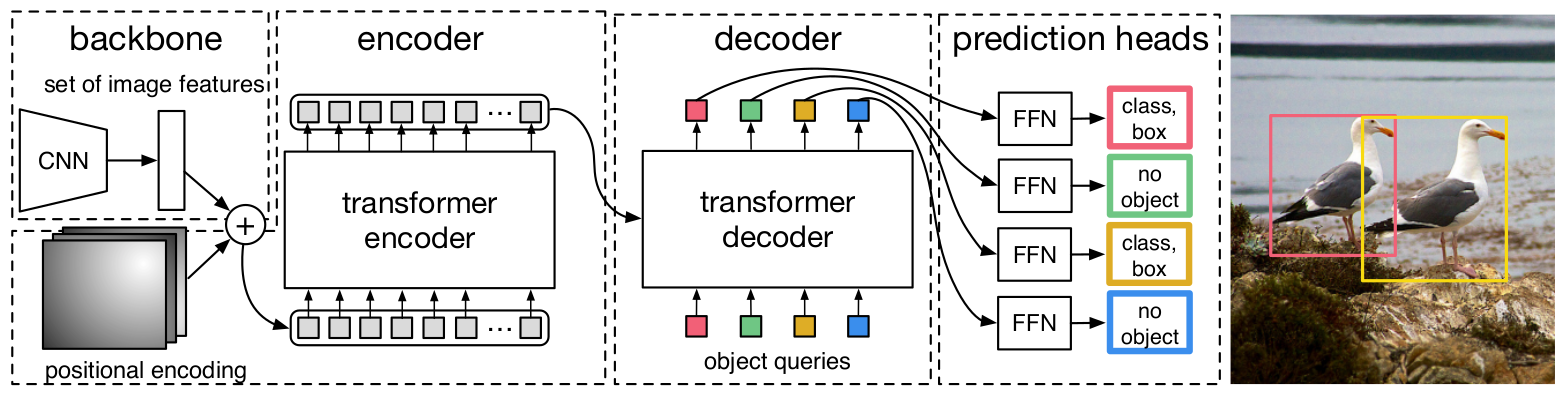
\includegraphics[width=\textwidth]{end_to_end_transformer}
%% \end{figure}


%% \begin{block}{Remarks}
%%   \begin{itemize}
%%   \item Convolutional layers are used to encode the image
%%   \item After a $1 \times 1$ convolutional layers, each feature map is flattened and considered as an input for the transformer encoder
%%   \item Decoder outputs are processed by a feed-forward network (FFN) to generate the box coordinates and label (possibly $\emptyset$).
%%   \end{itemize}
%% \end{block}

%% \end{frame}

%% %%%%%%%%%%%%%%%%%%%%%%%%%%%%%%%%%%%%
%% \begin{frame}{Results and comments}

%% \begin{itemize}
%% \item Similar accuracy and run-time performance to Faster R-CNN on the COCO object detection dataset
%% \item Optimization was apparently difficult (extra losses, for instance)
%% \end{itemize}

%% \begin{figure}[ht]
%%   \centering
%%   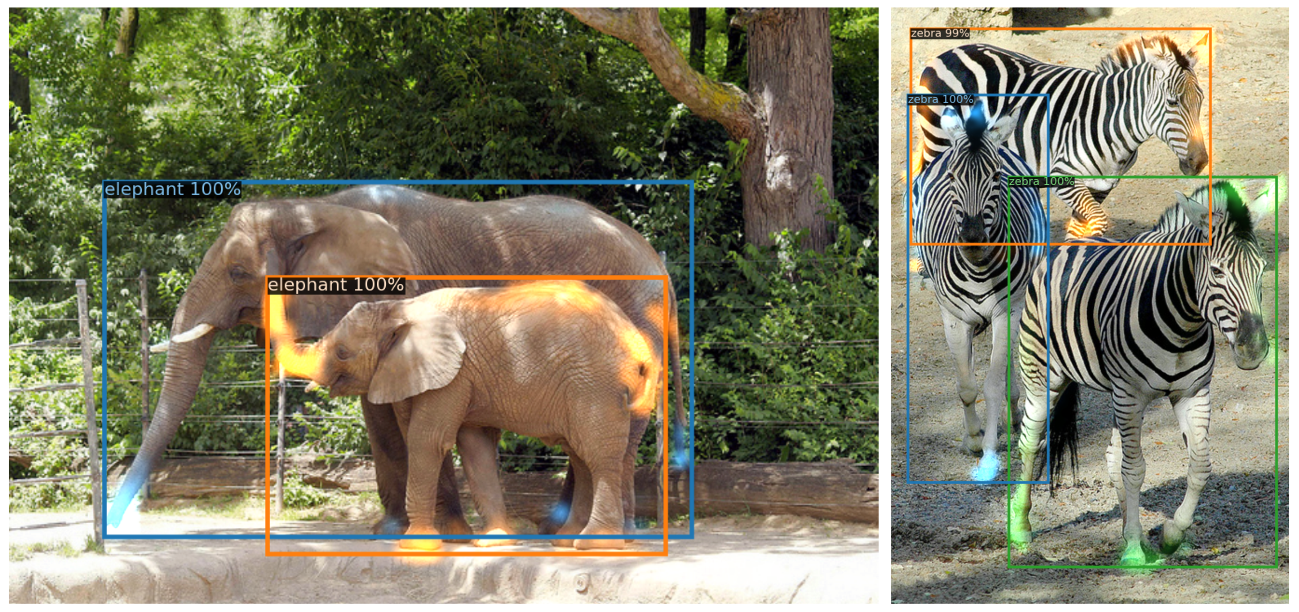
\includegraphics[width=0.8\textwidth]{detr_attention_scores}
%% \end{figure}


%% \end{frame}

%%%%%%%%%%%%%%%%%%%%%%%%%%%%%%%%%%%%
\subsection{Vision transformer}


%%%%%%%%%%%%%%%%%%%%%%%%%%%%%%%%%%%%
\begin{frame}{ViT: the vision transformer~\cite{dosovitskiy_image_2021}}

\begin{figure}[ht]
  \centering
  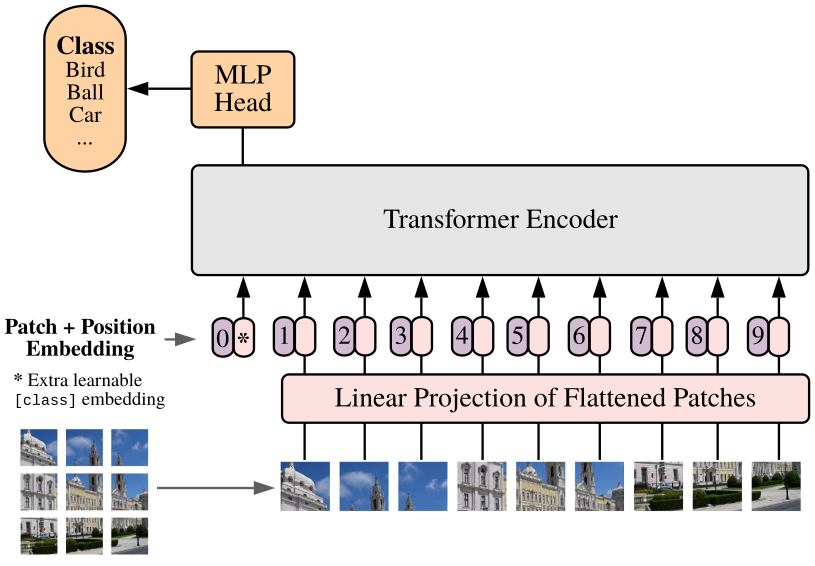
\includegraphics[width=0.6\textwidth]{vision_transformer}
\end{figure}

\begin{block}{Remarks}
  \begin{itemize}
  \item Only uses the transformer encoder
  \item Directly takes as inputs image patches
  \item Achieves state-of-the-art results when pre-trained on very large databases (Google's JFT-300M dataset)
  \end{itemize}
\end{block}


\end{frame}


%%%%%%%%%%%%%%%%%%%%%%%%%%%%%%%%%%%%
\begin{frame}{ViT results}

\begin{figure}[ht]
  \centering
  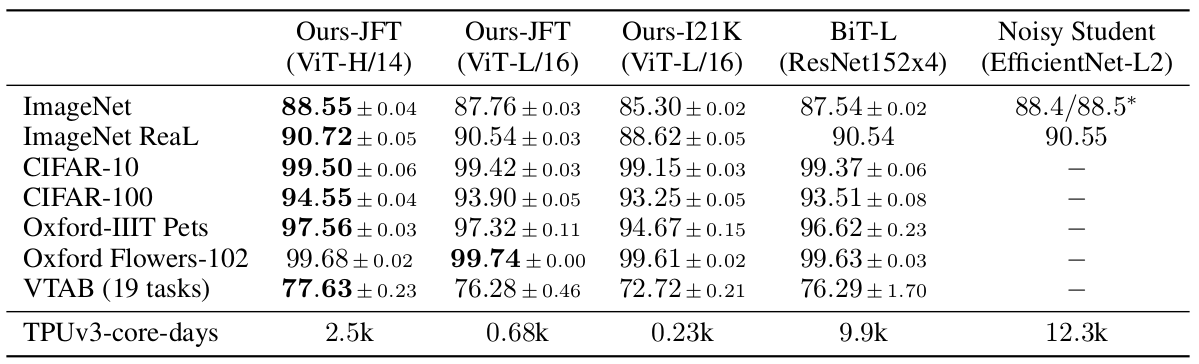
\includegraphics[width=\textwidth]{vit_table}
\end{figure}

\begin{block}{Remarks}
  \begin{itemize}
  \item Models pre-trained on JFT-300M
  \item Note the required processing power
  \end{itemize}

\end{block}

\end{frame}


%%%%%%%%%%%%%%%%%%%%%%%%%%%%%%%%%%%%
\begin{frame}{ViT results}

\begin{figure}[ht]
  \centering
  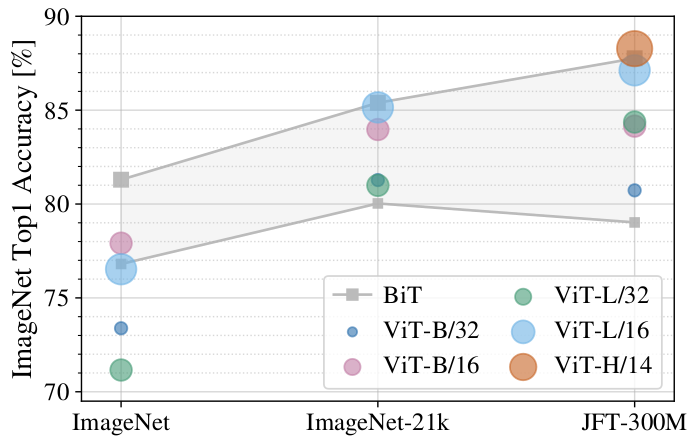
\includegraphics[width=0.6\textwidth]{vit_graph}
  \footnote{BiT: Big transfer~\cite{kolesnikov_big_2020}}
\end{figure}



\begin{itemize}
  \item ViT-H/14 requires 2500 TPUv3-core-days for pre-training
  \item But: ``Training data-efficient image transformers \& distillation through attention''~\cite{touvron_training_2021}.

\end{itemize}

\end{frame}


%%%%%%%%%%%%%%%%%%%%%%%%%%%%%%%%%%%%
\subsection{Shifted window transformer}

\begin{frame}{Shifted window (SWIN) transformer~\cite{liu_swin_2021}}


  \begin{columns}
    \begin{column}{.5\textwidth}
      \begin{figure}[ht]
        \centering
        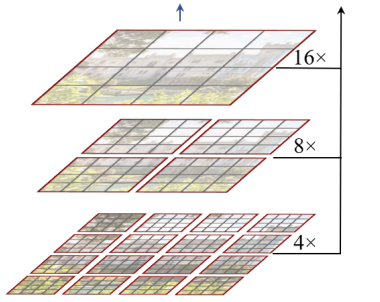
\includegraphics[width=\textwidth]{swin_hierarchy}
      \end{figure}

    \end{column}

    \begin{column}{.5\textwidth}
      \begin{itemize}
      \item The transformer modules are applied within each window
      \item Hierarchical approach: patches are merged at some levels
      \item The model uses \textbf{s}hifted \textbf{win}dows
      \end{itemize}
    \end{column}
  \end{columns}



\end{frame}

%%%%%%%%%%%%%%%%%%%%%%%%%%%%%%%%%%%%
\begin{frame}{SWIN blocks}

\begin{figure}[ht]
  \centering
  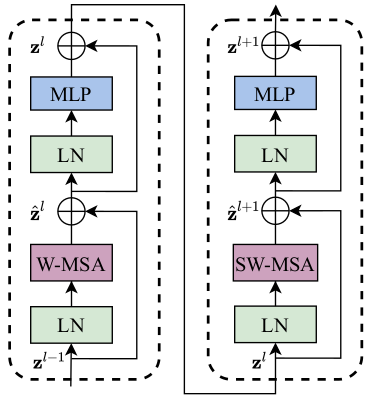
\includegraphics[width=.25\textwidth]{swin_blocks}
   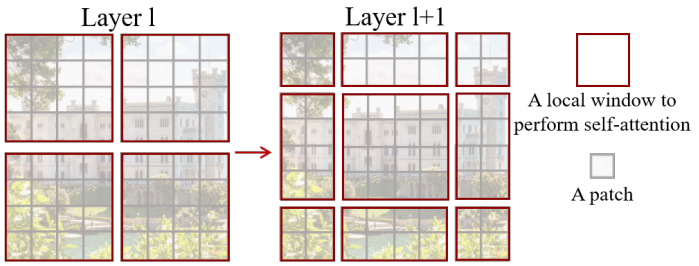
\includegraphics[width=.5\textwidth]{swin_windows}
\end{figure}

\begin{itemize}
\item Multi-headed self-attention with regular (W-MSA) and shifted  (SW-MSA) windowing configurations are applied alternatively
\end{itemize}

\end{frame}

%%%%%%%%%%%%%%%%%%%%%%%%%%%%%%%%%%%%
\begin{frame}{SWIN architecture }

\begin{figure}[ht]
  \centering
  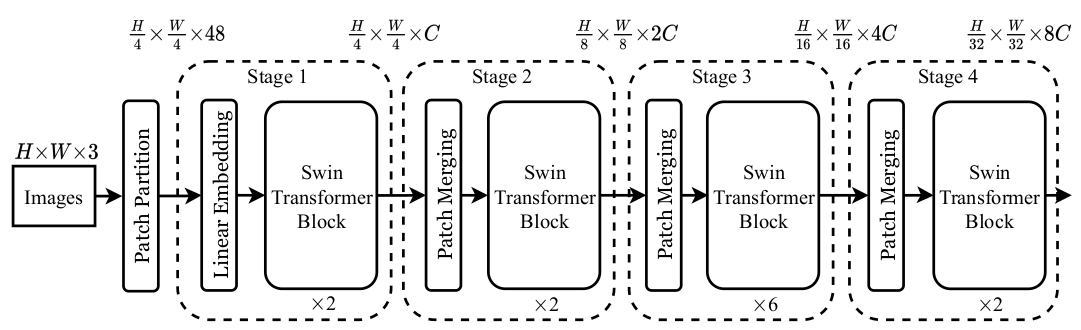
\includegraphics[width=\textwidth]{swin_archi}
\end{figure}

\begin{block}{Results}
  The Swin transformer obtains better results than previous methods on:

  \begin{itemize}
  \item ImageNet 1k and 22k classification
  \item COCO object detection and image segmentation
  \item ADE20k semantic segmentation
  \end{itemize}
\end{block}


\end{frame}

%%%%%%%%%%%%%%%%%%%%%%%%%%%%%%%%%%%%
\begin{frame}{Transformers chronology~\cite{amatriain_transformer_2023}}

\begin{figure}[ht]
  \centering
  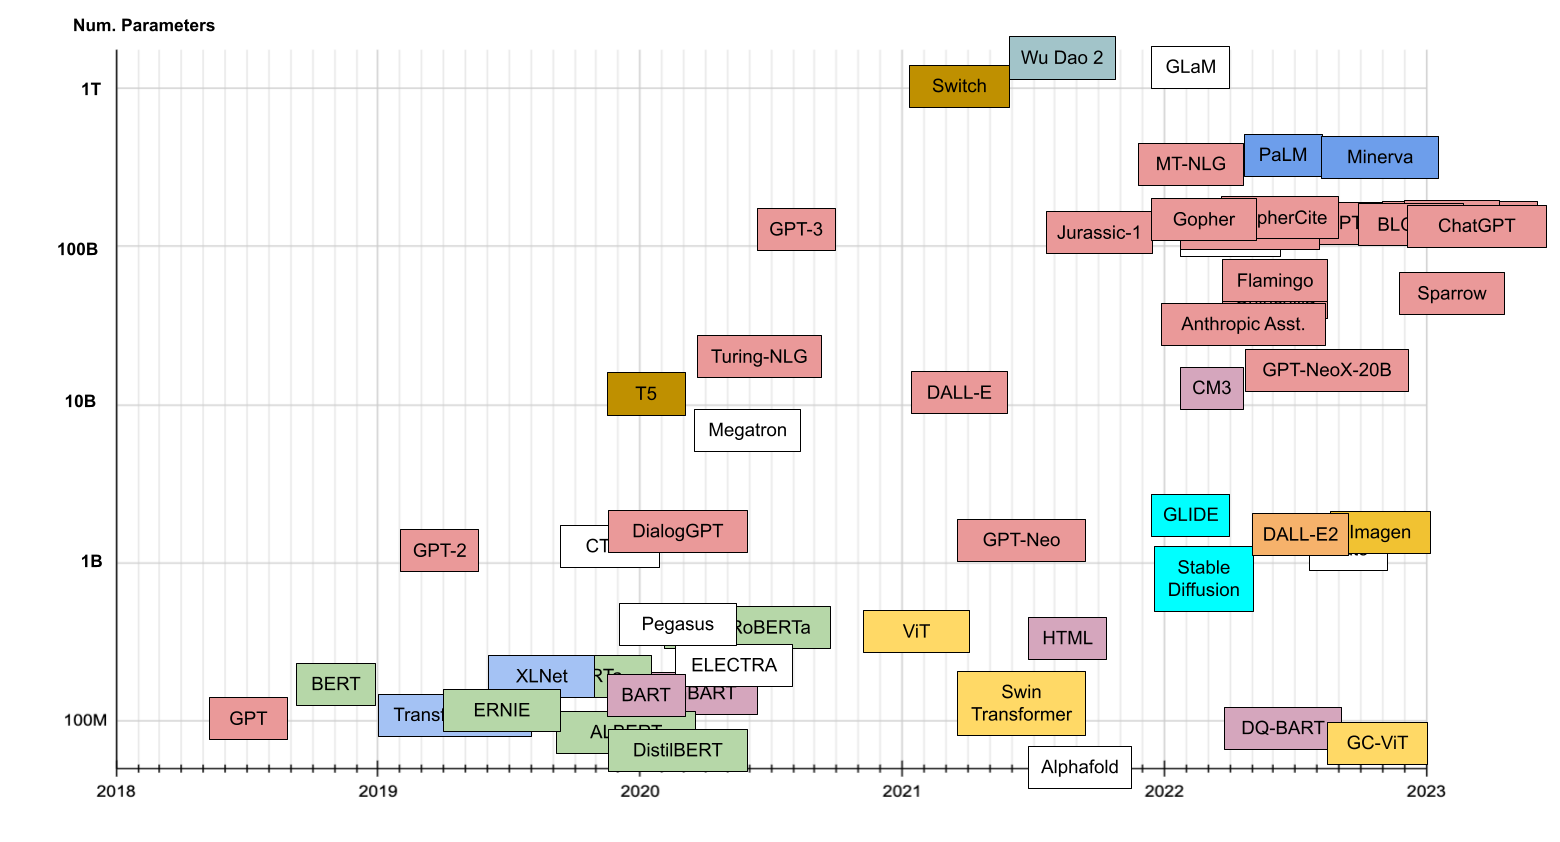
\includegraphics[width=\textwidth]{02-09}
\end{figure}


\end{frame}


%%%%%%%%%%%%%%%%%%%%%%%%%%%%%%%%%%%%
\subsection{Transformers for image segmentation}


\begin{frame}{TransUNet~\cite{chen_transunet_2021}}

\begin{figure}[ht]
  \centering
  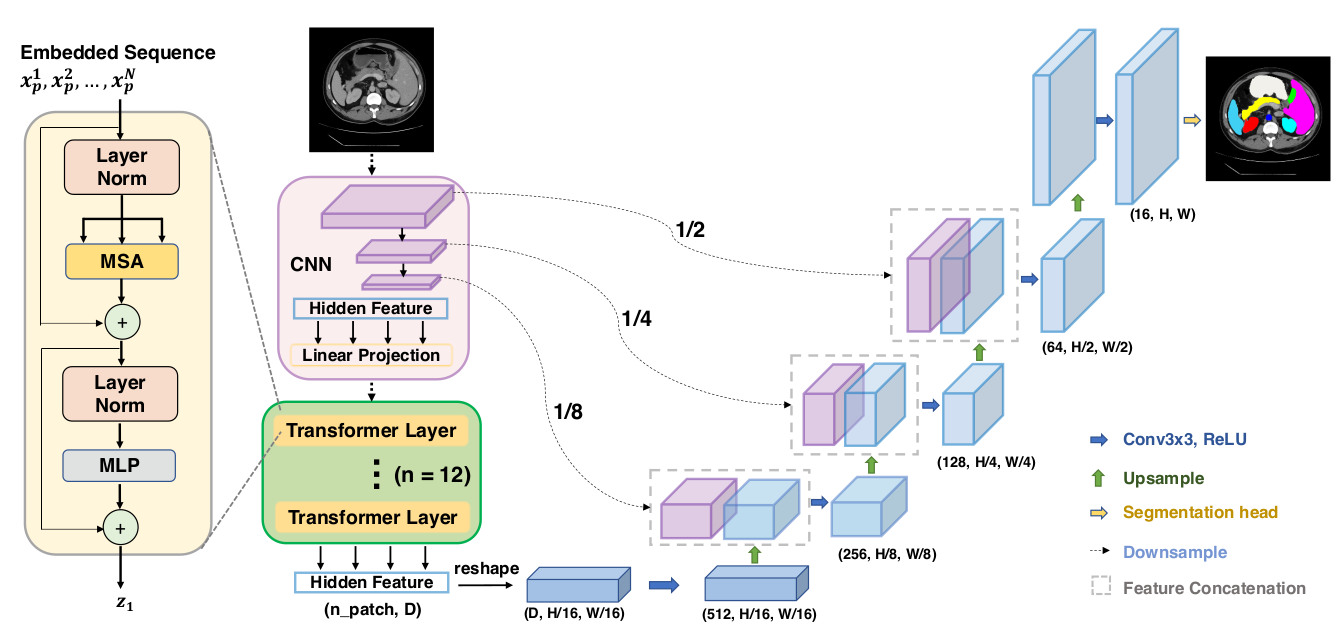
\includegraphics[width=\textwidth]{TransUNet}
\end{figure}


\end{frame}


%%%%%%%%%%%%%%%%%%%%%%%%%%%%%%%%%%%%
%%%%%%%%%%%%%%%%%%%%%%%%%%%%%%%%%%%%
\section{Discussion}

%%%%%%%%%%%%%%%%%%%%%%%%%%%%%%%%%%%%
\begin{frame}{Task: segment the rabbits that are in danger}

\begin{figure}[ht]
  \centering
  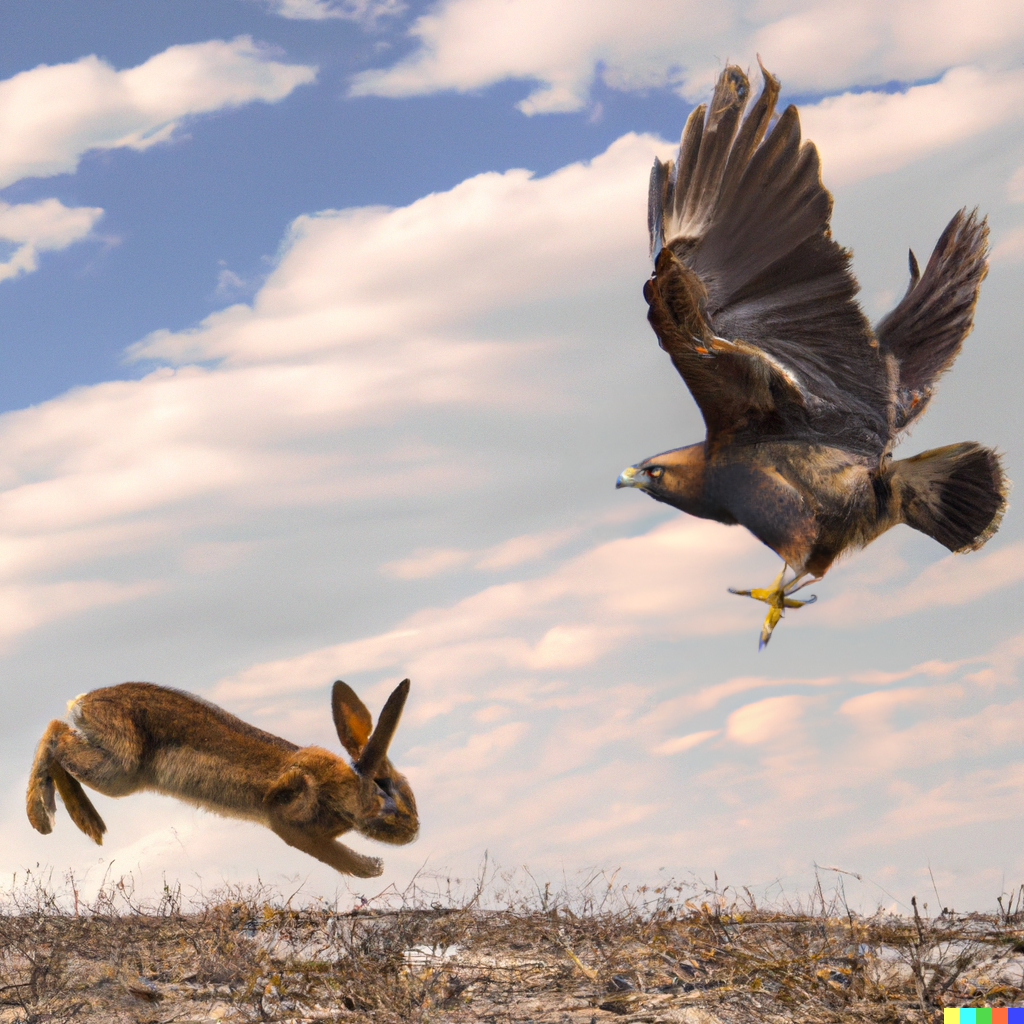
\includegraphics[width=0.4\textwidth]{DALLE2023-02-2311.39.20-An_eagle_flying_over_a_rabbit_photograph.png}
  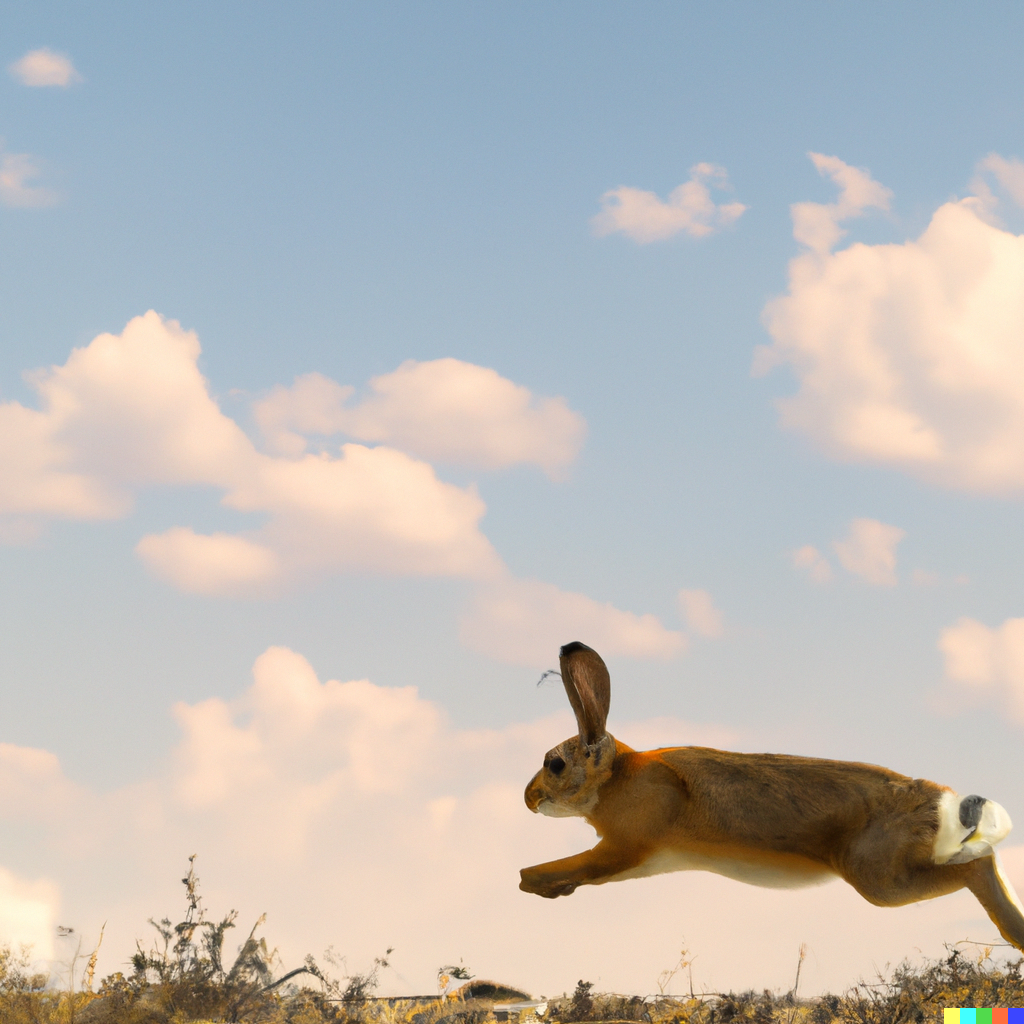
\includegraphics[width=0.4\textwidth]{DALLE2023-02-23-11.40.54-a_lonely_rabbit.png}
    \source{Images generated by DALL.E 2}
\end{figure}


\end{frame}



%%%%%%%%%%%%%%%%%%%%%%%%%%%%%%%%%%%%
\begin{frame}{Discussion}

  \begin{block}{Convolutional neural networks}

    \begin{itemize}[<+->]
    \item Convolutional networks are based on two inductive biases:
      \begin{itemize}
      \item Locality
      \item Translation equivariance
      \end{itemize}

    \item These hypothesis allow simplifying the models, but may also limit their generality

      \begin{itemize}
      \item Long range interactions are difficult to take into account
      \item Translation equivariance is not always welcome

      \end{itemize}
    \end{itemize}

  \end{block}

  \begin{block}{Transformers}

    \begin{itemize}[<+->]
    \item Transformers, like fully connected layers, do not make any assumptions on the data structure
      \begin{itemize}
      \item Localization is brought by a positional encoding
      \end{itemize}

    \item Are transformers a smart way of analysing images with fully connected layers?

    \end{itemize}
  \end{block}


\end{frame}


%%%%%%%%%%%%%%%%%%%%%%%%%%%%%%%%%%%%
\begin{frame}{MLPs is all you need~\cite{tolstikhin_mlp-mixer_2021}}

  \begin{figure}[ht]
    \centering
    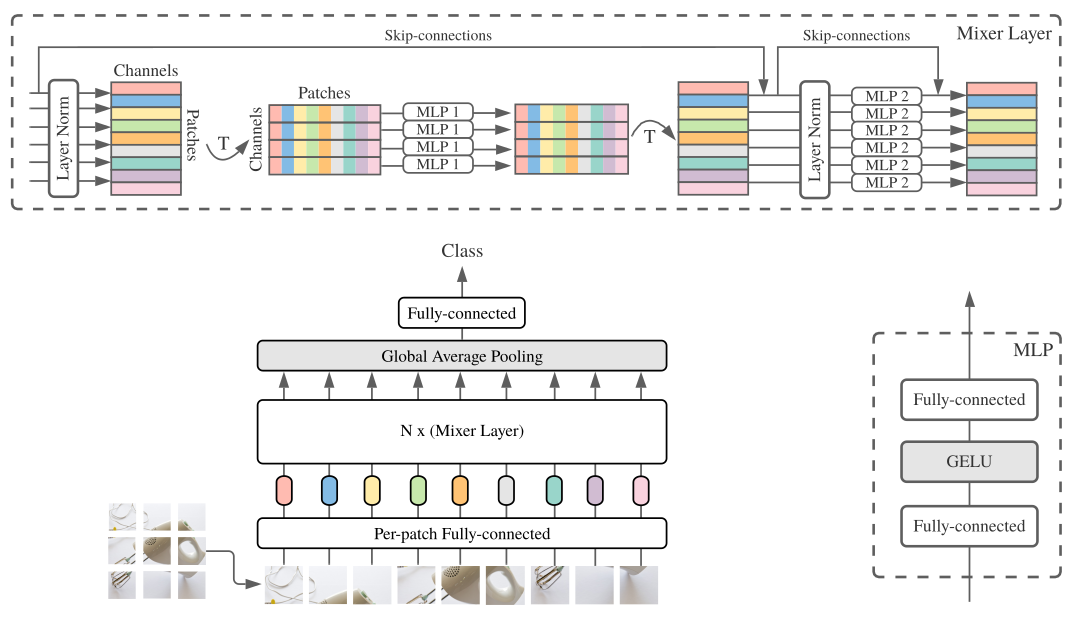
\includegraphics[width=\textwidth]{mixer}
  \end{figure}

\end{frame}


%%%%%%%%%%%%%%%%%%%%%%%%%%%%%%%%%%%%
%% \begin{frame}{Patches are all you need?~\cite{trockman_patches_2022}}

%% \begin{figure}[ht]
%%   \centering
%%   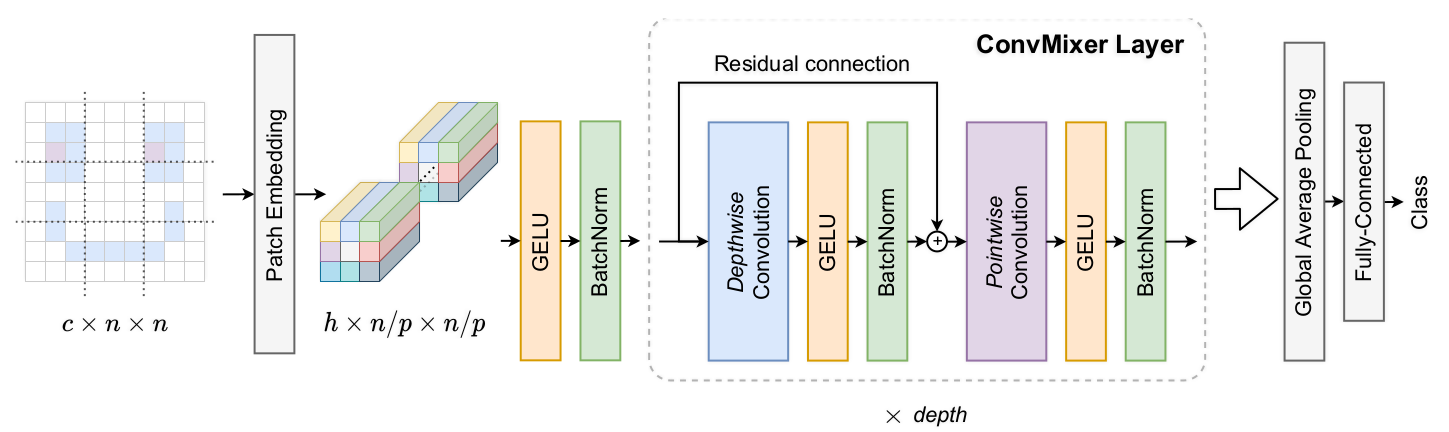
\includegraphics[width=\textwidth]{conv_mixer}
%% \end{figure}


%% \end{frame}

%%%%%%%%%%%%%%%%%%%%%%%%%%%%%%%%%%%%
\begin{frame}{And the winner is ...}

\pause

\begin{figure}[ht]
  \centering
  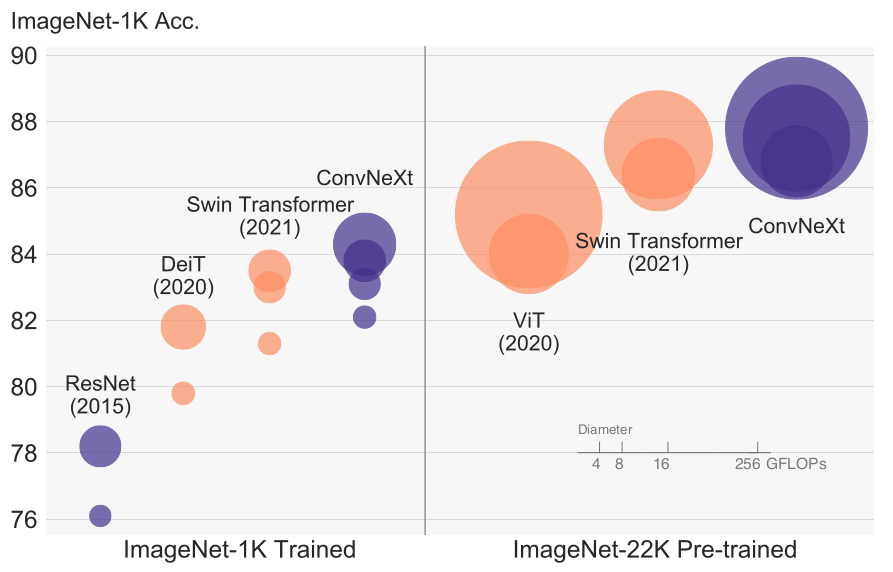
\includegraphics[width=0.8\textwidth]{convnext_vs_transformer}
\end{figure}

Competition is still ongoing~\cite{liu_convnet_2022}...


\end{frame}


%%%%%%%%%%%%%%%%%%%%%%%%%%%%%%%%%%%%
%% \begin{frame}{Announcement: internships with Mines Paris (CMM)}

%% \begin{itemize}
%% \item Exploring the latent space of scanning electron microscopy images of hair fibers. Industrial partner: L'Oréal. Location: Fontainebleau.
%% \item Apprentissage d’un observateur idéal pour la reconstruction 3D en vues éparses. Parner: CEA. Location: Saclay.
%% \item Acoustic image analysis for fish identification. Industrial partner: EDF. Location:  Chatou.
%% \item Stereo remote sensing. Industrial partner: Kadran (https://kadran-ingenierie.fr). Location: TBD.
%% \end{itemize}



%% \end{frame}


%%%%%%%%%%%%%%%%%%%%%%%%%%%%%%%%%%%%
%%%%%%%%%%%%%%%%%%%%%%%%%%%%%%%%%%%%%%%%%%%%%%%%%%
\section*{References}
%%%%%%%%%%%%%%%%%%%%%%%%%%%%%%%%%%%%%%%%%%%%%%%%%%

\frame[allowframebreaks]{

  \scriptsize

  \frametitle{References}

  %\bibliographystyle{amsalpha}
  %\bibliographystyle{apalike}

  \bibliography{../../edf.bib}

  \normalsize

}

\end{document}
